\documentclass[10pt,a4paper,twocolumn]{article}
\usepackage{textpos}
\usepackage{url}
\usepackage{graphicx}
\usepackage{array}
\usepackage{cite}
\usepackage{tikz}
\usetikzlibrary{shapes}
\usepackage{courier}
\usepackage[margin=1.0in, paperwidth=8.5in, paperheight=11in]{geometry}
\usepackage{amsmath}
\usepackage{amsfonts}
\usepackage{multirow}
\usepackage{subfigure}
\usepackage{enumitem}
\usepackage{chngcntr}
\counterwithin{figure}{section}
\counterwithin{table}{section}
\counterwithin{equation}{section}
\setlist[enumerate]{itemsep=0mm}
\setlist[itemize]{itemsep=0mm}
\newcommand{\fillin}[1]{X}
\newcommand{\mrow}[2]{\multirow{#1}{*}{#2}}

\begin{document}

\title{Neural Networks for Small-Scale Combat Optimization in Real-Time Strategy Games}
\author{Jacob Menashe and Vineet Keshari}
\maketitle

\begin{abstract}
A major challenge for players and AI modules alike in the real-time strategy community is the effective control of individual units in combat scenarios. Starcraft, a real-time strategy game released by Blizzard Entertainment, provides built-in heuristics for assisting players in combat management, but these heuristics are limited in their ability to make full use of a unit's potential. We present a series of techniques for training neural networks in small-scale combat situations, and lay the groundwork for further improvements to this system. We present a neural network design for controlling combat units, which, when coupled with the NEAT evolutionary learning algorithm, is able to consistently overcome Starcraft's built-in AI. In most cases our technique outperforms the AI in less than 100 generations, and scales to large battles in a variety of unit configurations. Our system achieves an 83\% win rate against the built-in AI, and a 50\% win rate against humans. We additionally lay out the groundwork to generalize our training method for competing against arbitrary opponents.
\end{abstract}

\section{Introduction}

Micro-management is a major component of real-time strategy (RTS) games such as Starcraft. Players must effectively move individual units around for gathering resources, constructing buildings, or for tactical combat. In the case of tactical combat, micro-management requires quick action on the part of the player and thus can be difficult to master even with a small number of units. While modern games tend to minimize the degree to which players must control units on a small scale through the implementation of batch commands, this is usually achieved with simple heuristics and a significant amount of potential is sacrificed for such enhancements. For a simple example of this, consider the following scenario: a player might take a heterogeneous group of close-range and long-range units and issue a batch attack command, at which point her units will either attack at random or attack one unit at a time. A more effective strategy might be to allow ranged units to disengage and re-engage based on the enemy's response, to allow these units to keep their distance, while close-range units focus on the greatest threat to allied ranged units. In this situation, the simplicity of the batch AI has diminished the effectiveness of the player's army. Such circumstances are prevalent in modern RTS games.

The domain of micro-management in combat environments is therefore well-suited to the application of intelligent, autonomous agents. While the best AI implementations still fall below the average competitive human player in terms of high-level planning and strategy \cite{weber2011building}, a trained unit controller agent should have little difficulty outperforming a human for any reasonably-sized army. Indeed, while an agent may potentially make hundreds of decisions and unit actions per second, even the most skilled human Starcraft players can only achieve about 5 actions per second \cite{mccoy2008integrated}.

In this paper we present a novel application of NEAT to small-scale combat problem, restricted to the domain of Starcraft. We devise a variety of network topologies and configurations for outperforming the game's built-in AI, as well as human players, and describe how our technique may be extended for outperforming winning bots from the Starcraft AI Competition \cite{ai_competition}. In Section \ref{sec:back} we discuss some background to AI development in real-time strategy games and specifically in Starcraft, and examine another body of work that focuses on small-scale combat. In Section \ref{sec:soft} we review the software libraries used for our analysis, and continue with a discussion of our approach to learning controller agents in Section \ref{sec:tech}. We evaluate our results against the built-in Starcraft AI, against other bots from the Starcraft AI Competition, and against other humans in Section \ref{sec:exp}. In Sections \ref{sec:conclusion} and \ref{sec:future} we conclude and discuss additional updates and improvements to our method, toward the ultimate goal of providing a general-use combat manager.

\section{Background}
\label{sec:back}

Classic AI techniques (or GOFAI) have been used on a variety of board games, such as Connect Four, Checkers, and Chess \cite{Allis94searchingfor}. Due to their simplistic and discrete state spaces, board games can often be broken down by traditional AI techniques such as alpha-beta pruning, or in some cases even brute force search. Chess pushes the limits of these techniques with a search tree complexity of at least $10^{120}$ \cite{Shannon:1988:PCP:61701.67002}, but can still benefit from the prediction value of limited search. What these games have in common is that computers maintain a significant advantage over humans stemming from their predictive abilities. As computing technology has improved, however, games have begun to take on more realistic simulations of the world and therefore rely heavily on continuous and highly complex states and actions. This increase in state-action complexity has in turn rendered traditional AI approaches ineffective at performing competitively with human opponents.

Recent work has seen reasonable success at taking on the challenges of modern games and simulations, particularly in the domain of First-Person Shooters (FPS). FPS games are a genre of computer game in which the player views the world through an avatar from a first-person point of view. The point of an FPS is to navigate through the game world and kill opponents with weapons and tools found throughout the environment. Neuroevolution has been successfully applied toward the goal of producing human-like actions \cite{schrum:cig11competition}, resulting in creating bots that effectively pass the Turing test. In FPS games, creating bots that are simply better than human players can be achieved through simple physics calculations, so here the emphasis is on enabling human-like movements and downgrading combat prowess where it can be seen as unrealistic. In contrast, our work focuses on outperforming human- and AI-controlled systems alike.

There has been considerable progress toward this goal in Starcraft, primarily due to the Starcraft AI Competition. The competition pits Starcraft bots against one another to determine a winner, however this task lies parallel to that of defeating a human controller. EISBot, one of the more successful bot implementations, has been tested against skilled human players and achieved a win rate of approximately 32\% \cite{weber2011building}. Other top-performing bots from the competition have been unable to win against expert players \cite{ai_comp_2010_website}. In our work, we therefore train and evaluate our networks based on the built-in AI, with the long-term goal of competing against both bots in the competition and human players.

Typical approaches to Starcraft bots include case-based reasoning \cite{weber2009case, weber2010case, cadena2011fuzzy} and hierarchical skill management \cite{mccoy2008integrated}. The former technique aims to learn skills, build order, and general strategy from replays of past games, while the latter technique organizes expert modules into a hierarchical decision model. These two approaches need not be mutually exclusive. Wender and Watson refine the problem of creating expert modules by focusing exclusively on small-scale combat tactics in \cite{rl_small_scale_combat}, and it is this work that relates most closely to our own. While Wender and Watson restrict their analysis to the particular combat configuration of a single, fast, ranged unit versus multiple slower short-ranged units, we seek to optimize small-scale combat in a more general sense by allowing for heterogeneous unit groups with an unspecified number of combatants. In this way, our approach moves toward a more flexible solution for the problem of micro-management in small-scale combat. 

Another notable difference between our work and that of \cite{rl_small_scale_combat} is our use of NEAT (see Section \ref{sec:neat}) for learning unit controllers. We select NEAT for a number of reasons. First, as we will describe in Section \ref{sec:net_design}, our state space is continuous and high-dimensional. Neural networks are naturally well-designed for parsing continuous state spaces and determining their value. Second, due to the computational cost of communicating with and executing commands on the Starcraft runtime, we are restricted in the number of iterations we may perform to learn this state space. NEAT has been shown to significantly outperform traditional reinforcement learning methods under these circumstances \cite{Stanley:2004:EEN:1048234}. Finally, while we can accurately determine the value of a match, we cannot predict what intermediate behaviors might be optimal for our overall goal of achieving combat prowess. We therefore rely on NEAT to discover these innovations in the form of connections and connection weights in an efficient manner.

\section{Software}
\label{sec:soft}

Our research was enabled by the BroodWar API (BWAPI) \cite{bwapi}, BWAPI Mono-Bridge \cite{monobridge}, and Starcraft: Broodwar itself. We use SharpNEAT \cite{sharpneat}, a C\# NEAT implementation for neuroevolution. While BWAPI is natively coded in C++, we selected a C\# implementation due to the following considerations:

\begin{itemize}
	\item Our focus for this work is in testing new configurations for NEAT and new combinations with our own heuristics, so development speed is of particular importance. C\# provides many high-level language features that allow for faster development than in C++.
	\item BWAPI only runs on Visual Studio in Windows, so there is no cross-platform or open-source advantage to using C++.
	\item SharpNEAT is an exceptionally well-coded and well-documented NEAT implementation. Along with working quite simply out of the box, the code is modularized and easily configurable, and has built in analysis and visualization tools.
\end{itemize}

Because C\# communicates with BWAPI through a client-server interface, processing is slower than would be in the case of C++. We felt that the increased productivity more than made up for this disadvantage.

It proved difficult to automate more complex training sessions due to the limitations of Starcraft and BWAPI. The Starcraft Campaign Editor has a number of bugs that prevent triggers from executing properly, forcing us to use a series of hacks to maintain quick training cycles. Automating bot-vs-bot battles was a challenge as well; the BWAPI software often crashes between battles, and is not fast enough for running the thousands of training rounds necessary for optimal results. For this reason, the majority of our training was performed against the built-in AI.

\section{Technical Approach}
\label{sec:tech}

We now cover our approach to the small-scale combat problem, beginning with a short introduction to NeuroEvolution of Augmenting Topologies (NEAT). We continue with a discussion of our implementation and network designs before proceeding to our software architecture.

\subsection{The NEAT Algorithm}
\label{sec:neat}

NEAT provides us with a fairly simple way of creating network designs without prior knowledge of the optimal target configuration. While traditional neural network algorithms such as backpropagation rely on a predefined network architecture, NEAT requires only that we specify a relatively small number of parameters. These parameters are shown in Table \ref{tab:neat_params}. Hidden nodes are added as needed based on random mutation and resulting fitness values.

\begin{table}
\centering
\begin{tabular}{|l|l|}
	\hline
	{\bf Parameter} & {\bf Interpretation}\\ \hline
	Input Nodes & State Representation\\ \hline
	Output Nodes & Actions and Decisions\\ \hline
	\multirow{2}{*}{Evolution Params} &  Intensity/Character of\\
	& Behavior Adjustments\\ \hline
\end{tabular}
\caption{Parameters specified for the NEAT algorithm.}
\label{tab:neat_params}
\end{table}

Properly designing the input and output nodes is critical to the performance of a neural network. We therefore maintain the evolutionary parameters defined in Table \ref{tab:neat_params_specific} for all tests, and instead focus our attention on the network I/O architecture.

\begin{table}
\centering
\begin{tabular}{|l|l|}
	\hline
	Connection Weight Mutation & 0.8\\ \hline
	Add Connection & 0.1\\ \hline
	Delete Connection & 0.001\\ \hline
	Add Node & 0.1\\ \hline
	Timesteps Per Activation & 10\\ \hline
	Connection Cycles & Enabled \\ \hline
\end{tabular}
\caption{Selected NEAT evolution probabilities. Values are normalized such that they sum to 1.0 upon evaluation.}
\label{tab:neat_params_specific}
\end{table}

\subsection{Training Setup}

Our network designs are closely tied to our training configurations, and thus we will cover the general outline for training to give context to our designs in following sections. Starcraft's built-in Campaign Editor application allows for users to create custom maps complete with environment specifications and state-based triggers. We used the campaign editor to construct scenarios in which teams of units are repeatedly spawned at two starting points, one for our bot (``allies") and one for the built-in AI (``enemies"). Allies and enemies repeatedly fight one another until all of one side has been defeated, signaling the completion of that round. For each genome generated by NEAT, we assign fitness based on its average performance over 5 rounds using Equation \ref{eqn:fitness}:

\begin{equation}
f = \frac{(A - E) * |(A - E)| + A_\mathrm{max}^2}{A_\mathrm{max}^2}\\
\label{eqn:fitness}
\end{equation}

where $A$ and $E$ are the ally and enemy counts at the end of the round, respectively, and $A_\mathrm{max} = E_\mathrm{max}$ is the starting count of allies or enemies in the training scenario. Using this formulation, the fitness value is always in the range $[0,2]$, with 1 representing a tie. In practice, ties only occur when the learned network moves the allies out of the combat area, so to avoid this behavior we assign a fitness score of 0 in all scenarios where $A \neq 0$ and $E \neq 0$.

\begin{figure}
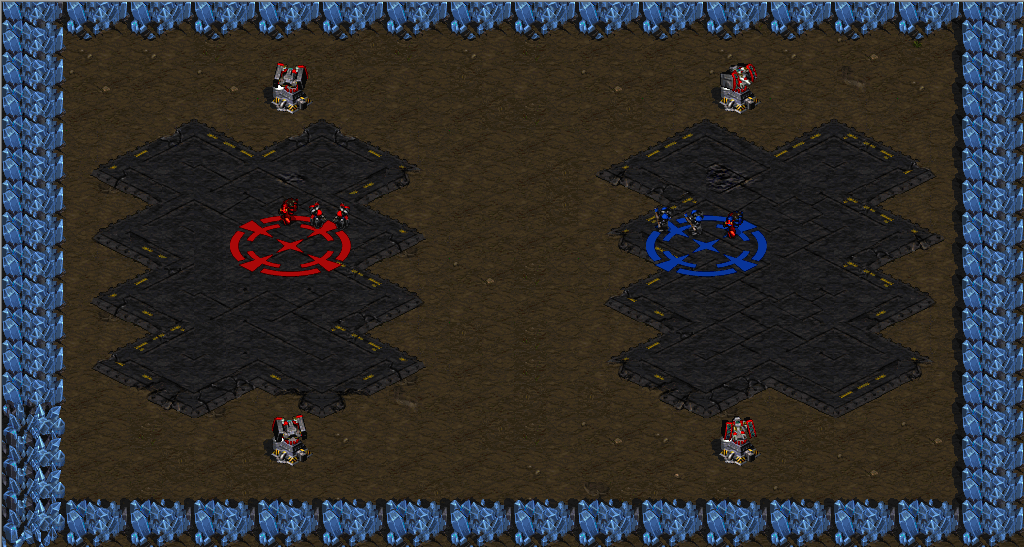
\includegraphics[scale=.28]{figures/mf_setup.png}
\caption{A screenshot of the Starcraft Campaign Editor setup for a 3v3 2-marine, 1-firebat training battle.}
\end{figure}


\begin{figure}
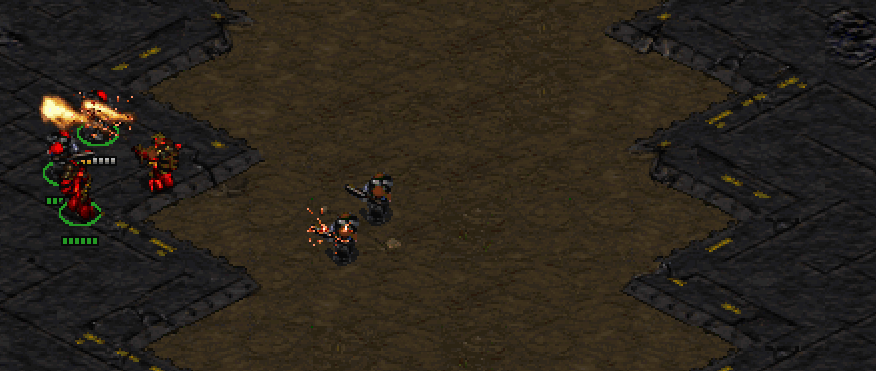
\includegraphics[scale=.34]{figures/mf_battle_small.png}
\caption{A 3v3 battle in the 2-marine, 1-firebat training battle.}
\label{fig:training_setup}
\end{figure}

\subsection{Network Design}
\label{sec:net_design}

We attempted multiple network designs, each of which is evaluated in Section \ref{sec:exp}. In this section we make multiple references to training time in terms of hours. Training was performed on a desktop PC with Starcraft and NEAT running on a single core at 3.07 GHz. 

\subsubsection{Multi-Unit Control}
\label{sec:multiunit_design}

We now begin with the multi-unit control network design in Figure \ref{fig:design_multiunit}.

\begin{figure}
\definecolor{turquoise}{RGB}{0,200,180}
\definecolor{orange}{RGB}{230,127,0}
\centering
\hspace*{-.5cm}
\begin{tikzpicture}[shorten >=1pt,->,draw=black!50, node distance=\layersep, scale=.8]
   \tikzstyle{every pin edge}=[<-,shorten <=1pt]
   \tikzstyle{neuron}=[circle,fill=black!25,minimum size=17pt,inner sep=0pt]
   \tikzstyle{input neuron}=[neuron, fill=green!50];
   \tikzstyle{output neuron}=[neuron, fill=red!50];
   \tikzstyle{hidden neuron}=[neuron, fill=blue!50];
   \tikzstyle{annot} = [text width=4em, text centered];
	\tikzstyle{health}=[rectangle,fill=green];
	\tikzstyle{ehealth}=[rectangle,fill=red];
	\tikzstyle{dist}=[rectangle,fill=blue];
	\tikzstyle{theta}=[rectangle,fill=blue];
	\tikzstyle{attack}=[rectangle,fill=orange];
	\tikzstyle{move}=[rectangle,fill=turquoise];

	\node[cloud, cloud puffs=15.7, cloud ignores aspect, minimum width=2cm, minimum height=5cm, align=center, draw] (hidden) at (2, 1.5) {};

    % Draw the input layer nodes
	\node[health] (ah1) at (0,4) {};
	\node[health] (ah2) at (0,3.5) {};
	\node[health] (ah3) at (0,3) {};
	\node[annot,left of=ah2, node distance = 1.5cm, text width = 2cm] (health_annot) {Ally \\ Health};
	\foreach \dest in {1,...,3}
		\path (health_annot) edge (ah\dest);

	\node[ehealth] (eh1) at (0,2) {};
	\node[ehealth] (eh2) at (0,1.5) {};
	\node[ehealth] (eh3) at (0,1) {};
	\node[annot,left of=eh2, node distance = 1.5cm, text width = 2cm] (ehealth_annot) {Enemy \\ Health};
	\foreach \dest in {1,...,3}
		\path (ehealth_annot) edge (eh\dest);

	\node[dist] (dist) at (0,0) {};
	\node[theta] (theta) at (0,-.5) {};
	\node[annot, text width = 2cm] (disttheta_annot) at (-2,-.25) {Enemy $r,\theta$ \\($\forall$ pairs)};
	\path (disttheta_annot) edge (dist);
	\path (disttheta_annot) edge (theta);

	\foreach \s in {ah1,ah2,ah3,eh1,eh2,eh3,dist,theta}
		\path (\s) edge (hidden);

	\node[attack] (a1attack1) at (4,4) {};
	\node[attack] (a1attack2) at (4,3.7) {};
	\node[attack] (a1attack3) at (4,3.4) {};

	\node[annot, text width=2.3cm] (a1attacks) at (5.6, 3.7) {Ally 1 Enemy Attack};

	\node[move] (a1moveScore) at (4,3) {};
	\node[move] (a1moveDist) at (4,2.7) {};
	\node[move] (a1moveTheta) at (4,2.4) {};
	\node[move] (a1moveFlip) at (4,2.1) {};

	\node[annot, text width=2.3cm] (a1moves) at (5.6, 2.4) {Ally 1 Move $(s,r,\theta,f)$};

	\node[annot, text width=.1cm] (dots) at (4,1.7) {\vdots};

	\node[attack] (a3attack1) at (4,1) {};
	\node[attack] (a3attack2) at (4,.7) {};
	\node[attack] (a3attack3) at (4,.4) {};

	\node[annot, text width=2.3cm] (a1attacks) at (5.6, .7) {Ally 3 Enemy Attack};

	\node[move] (a3moveScore) at (4,0) {};
	\node[move] (a3moveDist) at (4,-.3) {};
	\node[move] (a3moveTheta) at (4,-.6) {};
	\node[move] (a3moveFlip) at (4,-.9) {};

	\node[annot, text width=2.3cm] (a3moves) at (5.6, -.6) {Ally 3 Move $(s,r,\theta,f)$};

	\foreach \d in {a1attack1,a1attack2,a1attack3,a1moveScore,a1moveDist,
						a1moveTheta,a1moveFlip,a3moveScore,a3moveDist,
						a3moveTheta,a3moveFlip,dots}
		\path (hidden) edge (\d);

    % Annotate the layers
    \node[annot] at (0,5.2) {Input layer};
    \node[annot] at (2,5.2) {Hidden layer};
    \node[annot] at (4,5.2)  {Output layer};
\end{tikzpicture}

\caption{The multi-unit network design for 3 allies and 3 enemies. $r$ and $\theta$ represent relative distance and angle. $s$ represents a score in the range $[0,1]$, and $f$ is a flip.}
\label{fig:design_multiunit}
\end{figure}

This design represents our initial attempt at a network design. Inputs to the network include health percentages for each ally and each enemy in the training session, as well as the distances and angles of each enemy relative to each ally. Outputs include one score for each ally/enemy pair, as well as move score, distance, angle, and flip values for each ally. Flips are added as a way to differentiate between different extremes of the output range of the movement angle node. Originally we attempted a direct mapping of $\theta = 2 \cdot \pi \cdot o_\theta$, where $o_\theta \in [0,1]$ is the value of the movement angle output node. This has the effect that the extremes 0 and 1 map to the same movement. Thus, we instead use the following formulation:

 \begin{displaymath}
   \theta = \left\{
     \begin{array}{lr}
       o_\theta \cdot \pi & : f > 0.5\\
       o_\theta \cdot -\pi & : f \leq 0.5\\
     \end{array}
   \right.
\end{displaymath}

This way, units can move omnidirectionally with either extreme of the output range corresponding to different directions.

Using this network design, our units were able to achieve reasonable fitness levels in almost all trials with small combat scenarios within a few hours of training. Particularly, the design performed well with 3-5 units on either side. In the case of a 20-vs-20 battle, however, the design was not able to surpass an average population fitness of 1. This meant our units were losing battles more often than not, even after days of training. Reflecting on the design, this makes sense: with 20 allies and enemies there are $2 \cdot 20 + 20\cdot 20 \cdot 2 = 880$ input nodes and $20 \cdot (20 + 4) = 480$ output nodes. This results in over 400,000 possible connections, without taking into account hidden nodes that are added through neuroevolution. Given the constraints of interoperation with Starcraft, this presents a clear problem for quickly evolving networks to solve the small-scale combat problem. Moreover, the evolved networks are statically tied to the number of combatants; for any particular battle, we would need to have a precise controller pre-trained for that particular scenario. In practice, we would like our controllers to be more flexible, and thus we proceed to other solutions.

\subsubsection{Individual Control}
\label{sec:individual_design}

Our next attempt takes its inspiration from NERO \cite{stanley:ieeetec05}, where we use a single neural network design to control each combat unit individually. This allowed us to create more complex designs with the knowledge that we would not be restricted by the number of allied units in the training scenario. As we see in Figure \ref{fig:design_individual}, unit attributes are encoded into the inputs to allow for simultaneous learning on heterogeneous unit types. We furthermore use a polar map based on the idea of log-polar bins to represent enemy positions, health, and attributes. In this way, we allow for arbitrary configurations of heterogeneous enemy combatants. To reduce the number of output nodes, we use a small set of nodes for action selection, where the action with the highest score is selected. We then use another cluster of nodes for bin selection so that the highest-scoring action is applied to the target bin. Actions are defined in Table \ref{tab:actions}. Finally, to ensure that all values are normalized to the range $[0,1]$, each I/O value represents a percentage. Ally/Enemy counts are relative to the entire battle, so a bin with 7 enemies out of a total of 10 on the battlefield would have any enemy count value of 0.7, and a bin with all of the flying enemy units would have a \texttt{HasFlyer} value of 1.

\begin{figure}
\definecolor{turquoise}{RGB}{0,200,180}
\definecolor{orange}{RGB}{230,127,0}
\definecolor{purple}{RGB}{230,0,200}
\definecolor{urple}{RGB}{100,0,200}
\centering
\begin{tikzpicture}[shorten >=1pt,->,draw=black!50, node distance=\layersep]
   \tikzstyle{every pin edge}=[<-,shorten <=1pt]
   \tikzstyle{neuron}=[circle,fill=black!25,minimum size=17pt,inner sep=0pt]
   \tikzstyle{input neuron}=[neuron, fill=green!50];
   \tikzstyle{output neuron}=[neuron, fill=red!50];
   \tikzstyle{hidden neuron}=[neuron, fill=blue!50];
   \tikzstyle{annot} = [text width=4em, text centered];
	\tikzstyle{health}=[rectangle,fill=green];
	\tikzstyle{ehealth}=[rectangle,fill=red];
	\tikzstyle{dist}=[rectangle,fill=blue];
	\tikzstyle{theta}=[rectangle,fill=blue];
	\tikzstyle{action}=[rectangle,fill=orange];
	\tikzstyle{bin}=[rectangle,fill=turquoise];
	\tikzstyle{attr}=[rectangle,fill=purple];
	\tikzstyle{eattr}=[rectangle,fill=urple];

	\node[cloud, cloud puffs=15.7, cloud ignores aspect, minimum width=2cm, minimum height=5cm, align=center, draw] (hidden) at (2, 1.5) {};

    % Draw the input layer nodes
	\node[attr] (attr1) at (0,4) {};
	\node[attr] (attr2) at (0,3.7) {};
	\node[attr] (attr3) at (0,3.4) {};
	\node[annot, text width = 2cm] (attr_annot) at (-2,3.7) {Unit Attributes};
	\foreach \dest in {1,...,3}
		\path (attr_annot) edge (attr\dest);

	\node[health] (ah1) at (0,2.7) {};
	\node[health] (ac1) at (0,2.4) {};
	\node[ehealth] (eh1) at (0,2.1) {};
	\node[ehealth] (ec1) at (0,1.8) {};
	\node[annot, text width = 2.2cm] (allyenemy_annot) at (-2,2) {Ally/Enemy Health/Count Ratios ($\forall$ bins)};
	\foreach \d in {ah1,ac1,eh1,ec1}
		\path (allyenemy_annot) edge (\d);

	\node[eattr] (eattr1) at (0,0.9) {};
	\node[eattr] (eattr2) at (0,0.6) {};
	\node[eattr] (eattr3) at (0,0.3) {};
	\node[eattr] (eattr4) at (0,0.0) {};
	\node[annot, text width = 2.4cm] (eattr_annot) at (-2,.05) {Enemy Attributes  ($\forall$ bins)};
	\foreach \d in {1,...,4}
		\path (eattr_annot) edge (eattr\d);

	\foreach \s in {attr1,attr2,attr3,ah1,ac1,eh1,ec1,eattr1,eattr2,eattr3,eattr4}
		\path (\s) edge (hidden);

	\node[action] (action1) at (4,3) {};
	\node[action] (action2) at (4,2.7) {};
	\node[action] (action3) at (4,2.4) {};
	\node[action] (action4) at (4,2.1) {};
	\node[action] (action5) at (4,1.8) {};

	\foreach \d in {1,...,5}
		\path (hidden) edge (action\d);

	\node[annot, text width=2.3cm] (actions) at (6, 2.3) {Action Scores};

	\foreach \d in {1,...,5}
		\path (actions) edge (action\d);

	\node[bin] (bin1) at (4,0.1) {};
	\path (hidden) edge (bin1);

	\node[annot, text width=2cm] (bins) at (6, .1) {Bin Scores ($\forall$ bins)};
	\path (bins) edge (bin1);

    \node[annot] at (0,5) {Input layer};
    \node[annot] at (2,5) {Hidden layer};
    \node[annot] at (4,5)  {Output layer};
\end{tikzpicture}

\caption{The individual controller network design.}
\label{fig:design_individual}
\end{figure}

\begin{table}
\centering
\begin{tabular}{|l|l|}
	\hline
	{\bf Action Type} & {\bf Description}\\ \hline
	\texttt{AttackAir} & Attack air units\\ \hline
	\multirow{2}{*}{\texttt{AttackShort}} & Attack short-ranged \\
	& ground units\\ \hline
	\multirow{2}{*}{\texttt{AttackLong}} & Attack long-ranged \\ 
	& ground units\\ \hline
	\multirow{2}{*}{\texttt{AirBonus}} & Attack units that have a \\
	& bonus attack vs. air units\\ \hline
	\texttt{Move} & Move to target bin center\\ \hline
\end{tabular}
\caption{Discrete action types selected through competing output nodes.}
\label{tab:actions}
\end{table}

This network design performed well in a variety of scenarios, from small (3v3) battles to larger 20v20 battles, however the networks that were generated lost some of the interesting behaviors we had seen in the multi-unit controller. A side goal of our experiments was to create networks that discovered interesting behavior, and so we decided to try another formulation that combines the scalability of the individual unit controller with the enhanced awareness of the multi-unit controller. We examine this controller in Section \ref{sec:squad_design}.

\subsubsection{Squad Control}
\label{sec:squad_design}

\begin{figure}
\definecolor{turquoise}{RGB}{0,200,180}
\definecolor{orange}{RGB}{230,127,0}
\definecolor{purple}{RGB}{230,0,200}
\definecolor{urple}{RGB}{100,0,200}
\centering
\begin{tikzpicture}[shorten >=1pt,->,draw=black!50, node distance=\layersep]
   \tikzstyle{every pin edge}=[<-,shorten <=1pt]
   \tikzstyle{neuron}=[circle,fill=black!25,minimum size=17pt,inner sep=0pt]
   \tikzstyle{input neuron}=[neuron, fill=green!50];
   \tikzstyle{output neuron}=[neuron, fill=red!50];
   \tikzstyle{hidden neuron}=[neuron, fill=blue!50];
   \tikzstyle{annot} = [text width=4em, text centered];
	\tikzstyle{health}=[rectangle,fill=green];
	\tikzstyle{ehealth}=[rectangle,fill=red];
	\tikzstyle{dist}=[rectangle,fill=blue];
	\tikzstyle{theta}=[rectangle,fill=blue];
	\tikzstyle{action}=[rectangle,fill=orange];
	\tikzstyle{bin}=[rectangle,fill=turquoise];
	\tikzstyle{attr}=[rectangle,fill=purple];
	\tikzstyle{eattr}=[rectangle,fill=urple];

	\node[cloud, cloud puffs=15.7, cloud ignores aspect, minimum width=2cm, minimum height=5cm, align=center, draw] (hidden) at (2, 1.5) {};

	\node[health] (ah1) at (0,3.2) {};
	\node[health] (ac1) at (0,2.9) {};
	\node[ehealth] (eh1) at (0,2.6) {};
	\node[ehealth] (ec1) at (0,2.3) {};
	\node[annot, text width = 2.2cm] (allyenemy_annot) at (-2,2.5) {Ally/Enemy Health/Count Ratios ($\forall$ bins)};
	\foreach \d in {ah1,ac1,eh1,ec1}
		\path (allyenemy_annot) edge (\d);

	\node[eattr] (eattr1) at (0,0.9) {};
	\node[eattr] (eattr2) at (0,0.6) {};
	\node[eattr] (eattr3) at (0,0.3) {};
	\node[eattr] (eattr4) at (0,0.0) {};
	\node[annot, text width = 2.4cm] (eattr_annot) at (-2,.05) {Enemy Attributes  ($\forall$ bins)};
	\foreach \d in {1,...,4}
		\path (eattr_annot) edge (eattr\d);

	\foreach \s in {ah1,ac1,eh1,ec1,eattr1,eattr2,eattr3,eattr4}
		\path (\s) edge (hidden);

	\node[action] (action1) at (4,3) {};
	\node[action] (action2) at (4,2.7) {};
	\node[action] (action3) at (4,2.4) {};
	\node[action] (action4) at (4,2.1) {};
	\node[action] (action5) at (4,1.8) {};

	\foreach \d in {1,...,5}
		\path (hidden) edge (action\d);

	\node[annot, text width=2.3cm] (actions) at (5.6, 2.3) {Action Scores ($\forall$ allies)};

	\node[bin] (bin1) at (4,0.1) {};
	\path (hidden) edge (bin1);

	\node[annot, text width=2.4cm] (bins) at (5.6, .1) {Bin Scores \\($\forall$ bins, allies)};

    \node[annot] at (0,5) {Input layer};
    \node[annot] at (2,5) {Hidden layer};
    \node[annot] at (4,5)  {Output layer};
\end{tikzpicture}

\caption{The squad controller network design.}
\label{fig:squad_design}
\end{figure}

In Figure \ref{fig:squad_design} we see the basic design for the squad controller. The idea behind this design is to take a small number of predefined unit types and teach them to work together, so that they can be organized into a larger battalion with a squad commander. The network design is essentially a mix of the ideas from the multi-unit and individual-unit controllers: ally and enemy statistics are captured per bin (with respect to the squad's centroid), and action/bin scores are calculated for each ally. With 4 allies in one squad and 15 bins, this results in 105 input nodes and 80 output nodes.

\begin{figure}
\definecolor{turquoise}{RGB}{0,200,180}
\definecolor{orange}{RGB}{230,127,0}
\definecolor{purple}{RGB}{230,0,200}
\definecolor{urple}{RGB}{100,0,200}
\centering
\hspace*{-.5cm}
\begin{tikzpicture}[shorten >=1pt,->,draw=black!50, node distance=\layersep, scale=.8]
   \tikzstyle{annot} = [text width=4em, text centered];
	\tikzstyle{health}=[rectangle,fill=green];
	\tikzstyle{ehealth}=[rectangle,fill=red];
	\tikzstyle{move}=[rectangle,fill=orange];
	\tikzstyle{delegate}=[rectangle,fill=turquoise];
	\tikzstyle{count}=[rectangle,fill=urple];
	\tikzstyle{acount}=[rectangle,fill=urple];
	\tikzstyle{ecount}=[rectangle,fill=urple];

	\node[cloud, cloud puffs=15.7, cloud ignores aspect, minimum width=2cm, minimum height=5cm, align=center, draw] (hidden) at (2, 1.5) {};

	\node[health] (ah) at (0,3) {};
	\node[ehealth] (eh) at (0,2.5) {};
	\node[acount] (ac) at (0,1){};
	\node[ecount] (ec) at (0,.5){};

	\node[move] (m1) at (4,3) {};
	\node[delegate] (d1) at (4,0) {};

	\node[annot, text width=2.2cm] (health_annot) at (-2,3) {Ally, Enemy Health \% \\ ($\forall$ squads)};
	\node[annot, text width=2.2cm] (count_annot) at (-2,.75) {Ally, Enemy Count \% \\ ($\forall$ bins)};

	\node[annot, text width=3cm] at (5.65,3) {Move Score \\ ($\forall$ squads)};
	\node[annot, text width=3cm] at (5.65,0.2) {Delegate Score \\ ($\forall$ squads)};

	\path (health_annot) edge (ah);
	\path (health_annot) edge (eh);
	\path (ah) edge (hidden);
	\path (eh) edge (hidden);
	\path (count_annot) edge (ac);
	\path (count_annot) edge (ec);
	\path (ac) edge (hidden);
	\path (ec) edge (hidden);
	\path (hidden) edge (m1);
	\path (hidden) edge (d1);

    \node[annot] at (0,5.2) {Input layer};
    \node[annot] at (2,5.2) {Hidden layer};
    \node[annot] at (4,5.2)  {Output layer};
\end{tikzpicture}

\caption{The squad commander network design.}
\label{fig:quad_commander_design}
\end{figure}

Individual squads need to function together as a team, and thus we introduce the squad commander as the final network design we examined. The squad commander is much simpler than the other network designs, since it relies heavily on the fact that its squads are pre-trained. Figure \ref{fig:quad_commander_design} shows the details. The commander takes in ally and enemy health and positions, and decides whether to move each squad to a different location or to delegate control to that squad. The commander uses heuristics with prior knowledge to divide enemy groups between squads. For example, a squad that is well-equipped to take out flying units will preferentially be assigned flying enemy combatants as targets. Squads can therefore focus specifically on their targets assigned by the commander and ignore the rest of the enemies on the battlefield. This hierarchical organization reduces complexity at each level, and reduces overall design complexity by orders of magnitude.

\section{Experiments}
\label{sec:exp}

We now present a series of experiments to show the effectiveness of each network design in practice. In the following experiments we will refer to a handful of Starcraft units. These units are described briefly in Table \ref{tab:units}. We proceed with the experiments analogously to Section \ref{sec:net_design}, and conclude with small trials against an existing bot and a human competitor.

\begin{table}
\centering
\begin{tabular}{|l|l|}
	\hline
	{\bf Unit} & {\bf Description} \\ \hline
	Marine & Long-range ground unit \\ \hline
	\multirow{3}{*}{Firebat} & Short-range ground unit \\
	& Can hit multiple enemies \\
	& simultaneously \\ \hline
	\multirow{2}{*}{Ghost} & Long-range ground unit \\
	& More powerful than a marine\\ \hline
	\multirow{4}{*}{Goliath} & Long-range ground unit \\
	& Has attack bonus vs. air units \\
	& More powerful than marines, \\
	& firebats, and ghosts \\ \hline
	Wraith & Long-range air unit \\ \hline
\end{tabular}
\caption{Descriptions of units used in the training experiments.}
\label{tab:units}
\end{table}
	
\subsection{Multi-Unit Control}
\label{sec:multiunit_exp}

We performed our initial experiment to gauge the ability of a simple network design to outperform Starcraft's built-in AI. Using the controller from Section \ref{sec:multiunit_design} we construct a training scenario in which 2 marines and 1 firebat spawn for each team on the two sides of the combat area. The built-in (i.e. enemy) AI attacks the spawn location of the allied AI, ensuring that if the allies do nothing then a battle will still take place. Figure \ref{fig:multiunit_exp} shows the fitness graph obtained for this experiment.

Of particular interest in this experiment is the development of interesting behavior that was found. The first of these behaviors was a tendency for units to run away when only 1 ally is left in battle. Our original fitness formulation didn't assign any fitness value when battles ended due to a timeout. Due to the stochastic nature of these battles, a team with occasional wins could avoid losses entirely by running away when such a loss was imminent. The second interesting behavior regards the dynamics of firebats and marines. Firebats do a large amount of damage, so killing them as early as possible at as great a range as possible is preferable. In these training sessions we saw a behavior surface in which the allied firebat would go straight for the enemy firebat at the beginning of the battle, and then switch targets to a marine when the enemy firebat had gotten low on health. This dealt out a maximal amount of damage to the enemy firebat initially, while in some cases preserving the allied firebat in the process. It also ensured that allied marines could keep a safe distance from the enemy firebat. A video of this behavior is given in Table \ref{tab:videos}.

\begin{figure}
\centering
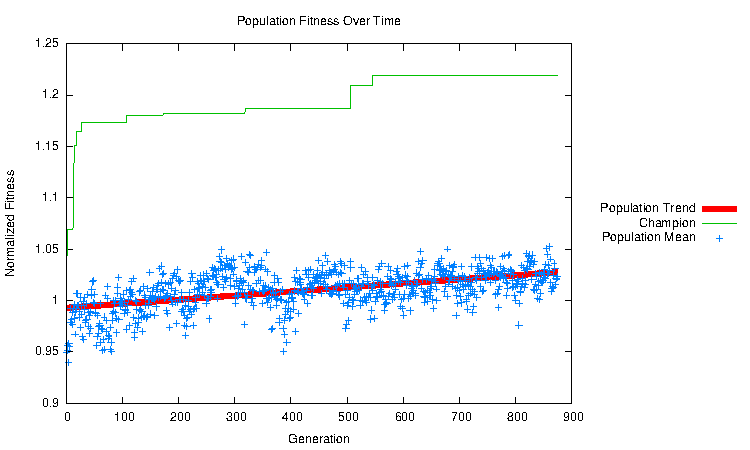
\includegraphics[scale=.59]{plots/multiunit.pdf}
\caption{A fitness graph of the multi-unit controller in a 3v3 scenario, with 2 marines and 1 firebat on each team. Mean population fitness progresses quickly toward a fitness score of about 1.2, indicating a strong advantage over the built-in AI.}
\label{fig:multiunit_exp}
\end{figure}

\subsection{Individual Control}

Our second experiment emphasizes the scalability of our individual unit controller described in Section \ref{sec:individual_design}. We use a 20-vs-20 training scenario in which each team has 5 ghosts, 5 firebats, 5 goliaths, and 5 wraiths. Figure \ref{fig:individual_exp} shows the fitness graph. This experiment differed from others in that no clear ``interesting" behavior was identified.

\begin{figure}
\centering
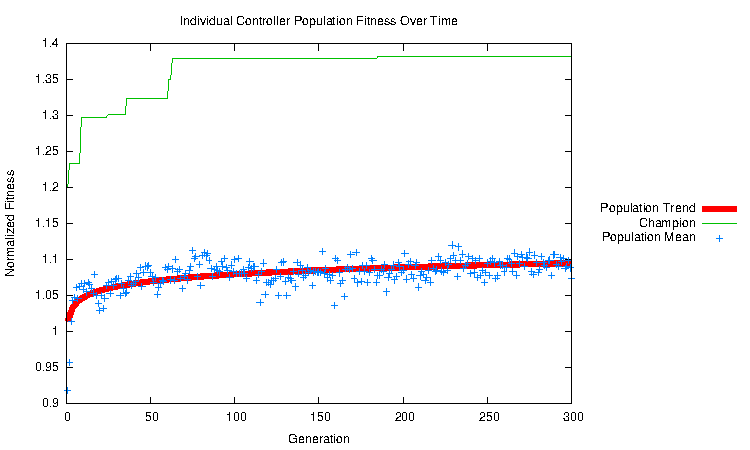
\includegraphics[scale=.59]{plots/individual.pdf}
\caption{A fitness graph of the individual-unit controller in a 20v20 scenario, with 5 ghosts, firebats, goliaths, and wraiths on each team. Fitness progresses rapidly in the first few generations, and then levels out over the next 300.}
\label{fig:individual_exp}
\end{figure}

Furthermore, we see a highly accelerated fitness gain during the first 4 generations. This is likely due to the mechanics of our network phenotypes. In the multi-unit controller, a unit can only move or attack a particular enemy, so each unit has a roughly 75\% chance of entering combat given a random genome. In the individual controller, the controller has the option of attacking different unit types. If a controller chooses to attack air units in a bin that doesn't have any, then no action is taken. Thus the individual controller encodes a large number of ``dead" actions. NEAT quickly learns to discard these state/action pairs. Once this has happened, evolution proceeds in roughly the same manner as in the multi-unit case, offset with a clear advantage over the built-in AI from the start. Considering its scalability and its improved fitness, the individual controller proves to be a significant improvement over the multi-unit controller.

\subsection{Squad Control}
\label{sec:squad_exp}

Motivated by our search for interesting behaviors, we now consider the squad controller and squad commander networks. The squad controller described in Section \ref{sec:squad_design} is somewhat of a hybrid between the multi-unit and individual controllers, combining the group awareness of the former with the flexibility and scalability of the latter. We trained two squad types with this controller: a 2-marine, 2-firebat controller, and a 2-goliath, 2-wraith controller. Fitness graphs for both of these are shown in Figures \ref{fig:squad_mf_exp} and \ref{fig:squad_gw_exp}. The marine-firebat setup performs poorly in comparison go the goliath-wraith setup, and the earlier marine-firebat controller from Section \ref{sec:multiunit_exp}. The multi-unit controller has a clear advantage in that it is highly specialized for the 2-marine, 1-firebat symmetric setup. Considering the high degree of similarity between the marine-firebat and goliath-wraith squad controllers, it's unclear why these two would achieve such varied fitness levels. One possible explanation is that stochasticity plays a larger role for ground units, whereas goliaths and wraiths are distinct enough that more optimization is possible from our state models.

\begin{figure}
\centering
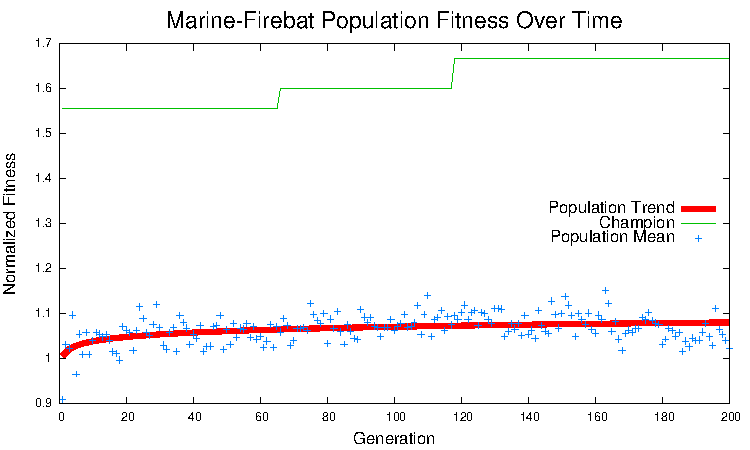
\includegraphics[scale=.59]{plots/squad_mf.pdf}
\caption{Fitness for the marine-firebat squad controller.}
\label{fig:squad_mf_exp}
\end{figure}

\begin{figure}
\centering
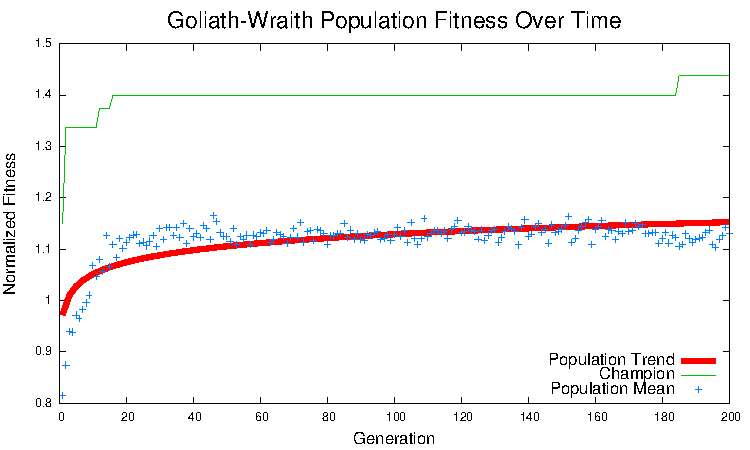
\includegraphics[scale=.59]{plots/squad_gw.pdf}
\caption{Fitness for the goliath-wraith squad controller.}
\label{fig:squad_gw_exp}
\end{figure}

Next we combine multiple squads into a single battalion using the squad commander network. We use a larger battle with 8 marines, 4 firebats, 4 goliaths, and 4 wraiths, to create 4 squads of 2-marine, 2-firebat groups, and 2 squads of 2-goliath, 2-wraith groups. The results are shown in Figure \ref{fig:squadcommand_exp}. While the squad controllers took approximately 6 hours for 300 generations, the squad commander required over 72 hours for 200 generations. The fitness graph closely follows a logarithmic trendline however, and extrapolation based on the trendline tells us that the genome will achieve a fitness score of 1.01 at 300 generations. This indicates more wins than losses, but is still behind the individual controller.

\begin{figure}
\centering
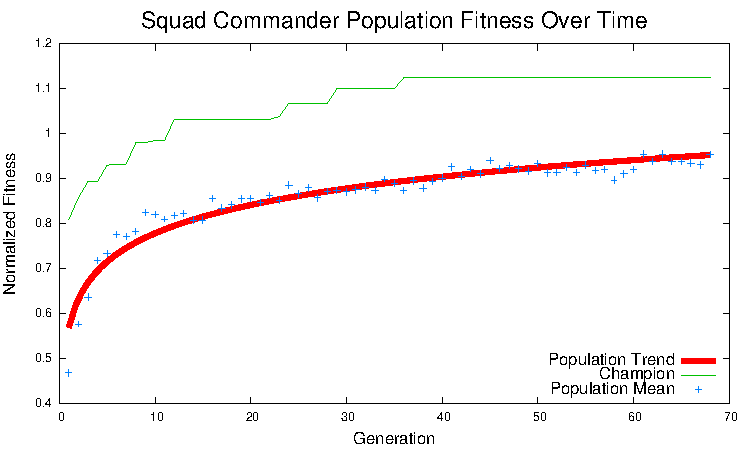
\includegraphics[scale=.59]{plots/squadcommand.pdf}
\caption{A fitness graph of the final squad commander network, using pretrained squad controllers from Figures \ref{fig:squad_mf_exp} and \ref{fig:squad_gw_exp}. Fitness is kept low, but increases more steadily after the initial few generations than with other controllers.}
\label{fig:squadcommand_exp}
\end{figure}

\section{Network Analysis}
\label{sec:network}

\begin{figure*}
\centering
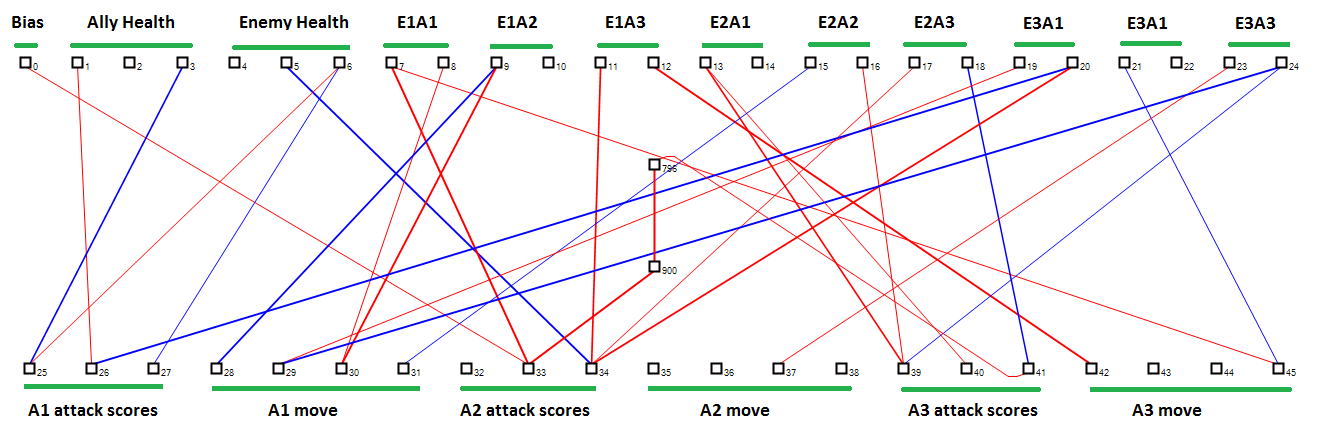
\includegraphics[scale=.5]{figures/multiunit_labelled.png}
\caption{The champion network for the multi-unit 2-marine, 1-firebat controller. Input nodes are at the top, hidden nodes in the middle, and output nodes at the bottom. Red lines represent positive connections, and blue lines represent negative connections. Green lines are used to label the grouped inputs and outputs as described in Section \ref{sec:network_struct}.}
\label{fig:multiunit_mf_net}
\end{figure*}

In this section, we will look at the champion network from the Marine2Firebat1 multi-unit controller shown in Figure \ref{fig:multiunit_mf_net} and analyze any interesting behavior that it has evolved during training. We choose to study this network as it has the least number of nodes amongst our various approaches, making it easier to visualize and to infer behavior. Our aim in this section is to understand whether or not the better fitness is indeed due to intelligent behavior.

\subsection{Network Diagram}
\label{sec:network_struct}

The network diagram in Figure \ref{fig:multiunit_mf_net} was generated from trained genomes using the SharpNEATView library \cite{sharpneat}. Node 0 is the bias, while nodes 1 to 24 and 25 to 45 are the inputs and outputs of the network respectively, arranged as per the network structure shown in Figure \ref{fig:design_multiunit}. The units in our training setup are labelled A1-A3 and E1-E3 as per Table \ref{tab:multiunit_labels}. Inputs 7 to 24 are the \{r,$\theta$\} values for the relative positions of each enemy-ally pair. The angle $\theta$ is in world co-ordinates, so that $\theta$=0 is to the right in the training setup shown in Figure \ref{fig:training_setup}. The `move' outputs in order for each ally are the move score, distance, $\theta$ and flip, as described in Section \ref{sec:multiunit_design}. We will denote a connection as \{(source node):(destination node)\} in the following subsections.

\begin{table}
\centering
\begin{tabular}{|l|l|}
	\hline
	{\bf Label} & {\bf Unit} \\ \hline
	A1 & Marine 1 \\ \hline
	A2 & Marine 2 \\ \hline
	A3 & Firebat \\ \hline
	E1 & Enemy Marine 1 \\ \hline
	E2 & Enemy Marine 2 \\ \hline
	E3 & Enemy Firebat \\ \hline
\end{tabular}
\caption{Labels for units in the network shown in Figure \ref{fig:multiunit_mf_net}.}
\label{tab:multiunit_labels}
\end{table}

\subsection{Network Behavior}
\label{sec:network_behavior}

Based on initial configuration in our training setup, at the beginning of a round both marines will attack E2, while the Firebat will go for E1. The Firebat's behavior is useful since the enemy marines can cause a lot of damage to it due to their long range. It is also beneficial for both marines to focus attack on a single enemy so that they can kill it early, reducing the total damage taken by the team thereafter. Connections \{1:26\}, \{0:33\}, \{7:33\} and \{13:39\} contribute to these behaviors. Further behavior is described for each unit in the following subsections.

\subsubsection{Marine 1 (A1)}
\label{sec:network_out_a1}

A1 will attack E2 as long its own health percentage is high. As its health drops after initial conflict, its preferences for enemies depend on the enemy firebat's health. If the enemy firebat is weak, A1 will attack it to kill it quickly due to \{6:27\}. If the enemy firebat is stronger than the ally firebat, A1 will instead attack E1 (\{3:25\} and \{6:25\}). This may be because E1 is the likely cause of higher damage to the ally firebat at this point as E2 should have been killed early.

\subsubsection{Marine 2 (A2)}
\label{sec:network_out_a1}

A2 has a predisposition to attack E2 due to \{0:33\}. This preference is further increased if our firebat is attacking the enemy firebat, as given by the connection chain \{41:796:900:33\}. A2 can be seen as protecting the firebat from damage from E2 in this behavior. However, if E2's health is low enough and both enemy marines are away from our firebat (thereby posing no threat to it), A2 will instead attack the enemy firebat due to \{5:34\}, \{11:34\} and \{17:34\}. This is the reverse of the previous behavior, where A2 tries to take advantage of its range to attack the enemy firebat.

\subsubsection{Firebat (A3)}
\label{sec:network_out_a1}

The Firebat's behavior is influenced more by the angles between allied and enemy units than it is by their health or relative distances. It can be said that A3 is more sensitive to the spatial configuration of units on the battlefield than are the marines. It is difficult to quantify this behavior due to the linear nature of the values for $\theta$ in the multi-unit controller network, as opposed to the use of discrete bins in the others. We can, however, make a guess at what these connections mean based on our observations. A3's initial tendency to attack E1 will be reduced if the enemy firebat makes a large angle to it (\{24:39\}). This is usually the case in our training setup, as the enemy firebat always spawns at the lower right corner. Due to this, A3 may have a stronger tendency either to attack E2 if it is not close to A1 (\{13:40\}), or to attack E3 if the angle between A3 and E2 is small (\{18:41\}). In most cases, the latter scenario occurs due to the way the units spawn (A3 in the lower left corner, E3 in the lower right corner and E2 somewhere above E3). We therefore observe that A3 initially attacks E1 but when the units get closer it may attack E3. In either scenario, however, the firebat will first damage an enemy marine and then the enemy firebat.

\subsection{Remarks}
\label{sec:network_remarks}

While we can show signs of intelligent behavior from the champion network's structure and performance, it should be noted that the network is far from perfect. Many of the connections do not contribute to useful behavior, while many that should are not present (e.g. a marine can retreat when the enemy firebat gets close). The two hidden nodes in two layers are also redundant, as they form a chain of positive weights and can be replaced with a single connection \{41:33\}. This is because the network, while effective, was still going through the evolution process when this genome was evaluated. We stopped training the network once a reasonable level of fitness was attained due to time constraint, but further iterations through hundreds of generations may have resulted in more focussed behavior as well as higher fitness.

\section{Combat Results}

To anchor our reported fitness scores to a practical setting, we now present results for a variety of controllers and training scenarios. These are given in Table \ref{tab:results}. We include tests against the Skynet bot \cite{skynet}, the current champion of the Starcraft AI competition. Skynet only performed reliably in our 20v20 large-scale battle. In small-scale battles, the units acted erratically.

\begin{table*}
\centering
\begin{tabular}{|c|c|c|c|c|}
	\hline
	{\bf Game} & {\bf Players } & {\bf Fitness $\mu$} & {\bf Fitness $\sigma$} & {\bf Wins - Losses } \\ \hline
	MFGW 20v20 & SC vs. BWAI & 0.94 & 0.16 & 740 - 1260 \\ \hline
	Heterogeneous 20v20 & IC vs. BWAI & 1.11 & 0.21 & 1,661 - 339\\ \hline
	Heterogeneous 20v20 & IC vs. Skynet & 0.76 & 0.24 &  160 - 1,840 \\ \hline
	Heterogeneous 20v20 & IC\textsuperscript{$\prime$} vs. Skynet & 0.81 & 0.23 & 94 - 906 \\ \hline
	Heterogeneous 20v20 & IC (untrained) vs. Skynet & \fillin{mean} & \fillin{stddev} & \fillin{results} \\ \hline
	Heterogeneous 20v20 & IC vs. Human & 0.96 & 0.19 & 4 - 6 \\ \hline
	Heterogeneous 20v20 & Human vs. Skynet & N/A & N/A & 4 - 6 \\ \hline
	2-Goliath, 2-Wraith & Human vs. BWAI & N/A & N/A & 9 - 1\\ \hline
	2-Goliath, 2-Wraith & SC vs. Human & 0.96 & 0.16 & 5 - 5 \\ \hline
	2-Marine, 1-Firebat & MUC vs. BWAI & 1.17 & 0.35 & 1495 - 515 \\ \hline
\end{tabular}
\caption{The final results for a selected set of genomes. Only completed games are reported, and wins/losses are reported with respect to the first player listed. MUC, IC, SC, and BWAI represent Multi-Unit Controllers, Individual Controllers, Squad Controllers, and the built-in BroodWar AI, respectively. MFGW refers to the marine-firebat-goliath-wraith setup described in Section \ref{sec:squad_exp}. Unless otherwise noted, all controllers were trained against BWAI and sample from a trained population. IC\textsuperscript{$\prime$} is identical to IC, except its population is trained against Skynet as well.}
\label{tab:results}
\end{table*}

\begin{table*}
\centering
\begin{tabular}{|l|l|l|}
	\hline
	{\bf Video} & {\bf Players} & {\bf Description}\\ \hline
	\mrow{2}{\small \url{http://youtu.be/OeMwC0bexlo}} & \mrow{2}{MUC vs. BWAI} & 3v3 battle with 2 marines and \\
	&& 1 firebat on each team\\ \hline
	\mrow{2}{\small \url{http://youtu.be/zHyUqjc55Bc}} & \mrow{2}{IC vs. BWAI} & 20v20 battle with heterogeneous \\
	&& units, using an individual controller. \\ \hline
	\mrow{2}{\small \url{http://youtu.be/07mQnSVvytU}} & \mrow{2}{IC\textsuperscript{$\prime$} vs. Skynet} & 20v20 battle against Skynet with \\
	&& heterogeneous units. \\ \hline
	\mrow{2}{\small \url{http://youtu.be/2IKllwxzlGA}} & \mrow{2}{SC vs. BWAI} & 20v20 battle against BWAI with the \\
	&& marine-firebat-goliath-wraith setup. \\ \hline
\end{tabular}
\caption{A collection of videos displaying the training battles. MUC, IC, SC, and BWAI represent Multi-Unit Controllers, Individual Controllers, Squad Controllers, and the built-in BroodWar AI, respectively. IC\textsuperscript{$\prime$} was trained additionally against Skynet.}
\label{tab:videos}
\end{table*}

The results show that while our bots do indeed perform well against the built-in AI, this expertise doesn't generalize to human players or the Skynet bot. To improve performance against Skynet, we trained our individual controller population against Skynet. This training session was exceptionally processor-intensive. While 3v3 scenarios trained at approximately 12.5 generations per hour, we were able to achieve less than one generation per hour against Skynet. We therefore trained the IC controller for 15 additional generations against the Skynet bot. The fitness improvement is small but significant ($p < .001$), indicating that learning is taking place and that our network could potentially overcome the Skynet bot given weeks of training.

\section{Conclusions}
\label{sec:conclusion}

We have shown the effectiveness of three different approaches to creating small-scale combat controllers using neural networks and NEAT to learn control techniques. In each case we have shown that given the proper training setup, these designs are capable of performing well against the built-in AI. We additionally show that our method is competitive against a human player, and while the top-ranking AI still outperforms our most successful genome, it's possible that continued training against Skynet could change these results. We discuss this and further modifications to our methods in the final section.

\section{Future Work}
\label{sec:future}

The most obvious deficiency of our training method is the reliance upon Starcraft's built-in AI for training. This AI is rather poor at small-scale combat, and so our best genomes were only barely competitive in human trials and were easily defeated against Skynet. Training directly against a target opponent (such as Skynet) seems like a reasonable requirement at the surface, however we would prefer a system that does not rely on prior knowledge of the opponent's behaviors and tendencies. Therefore a possible remedy to this would be a competitive evolutionary setup, in which our genomes compete against one another. This would push for continual innovation, and we believe would allow for better generalization against unknown bots or human opponents. Allowing for this type of evolutionary strategy would require updates to BWAPI to allow smoother transitions between battles in a multi-instance setting. Alternatively, our system could be moved off of the BWAPI platform and onto an open-source alternative, such as ORTS \cite{orts}.

Another possible area of improvement lies in squad command and enemy grouping. Our current squad commander implementation relies on hard-coded heuristics for grouping squads with enemies. An alternative approach might use the neural network controlling the squad commander to make these decisions as well. Rather than ignoring enemy attributes and simply choosing to move or delegate, the commander might learn to associate enemy configurations with a library of trained squads. Squads can be trained effectively in just a few hours on a standard desktop machine, allowing for a large number of specialized squads to be created for the commander to choose from.

Our current implementation also does not make use of specialized unit abilities. For example, a Templar unit is able to use the Psionic Storm ability to attack a large area of enemies simultaneously. Effective use of these abilities is a particular challenge for human players, so mastering them would prove a significant advantage for an AI controller. Using the squad paradigm, it would be a simple matter to attach unique unit abilities to individual squads without a significant increase in training complexity.

Finally, the squad commander network should be more flexible to different squad configurations. This might be achieved by discretizing squad attributes with adjectives like \texttt{HasAttackAirBonus} or \texttt{CanTurnInvisible}. This would add invariance to squad ordering and specific setup by instead focusing on each squad's abilities. To handle varying numbers of squads, we propose a recursive hierarchical structure like the squad commander/controller setup we use here, in which multiple layers of combat strategy oversee the course of a battle. This corresponds to real-world combat scenarios in which officer ranks determine each soldier's level of oversight.
	
\bibliographystyle{unsrt}
\bibliography{bibliography}

\end{document}